\chapter{Elixir}
Elixir is a dynamic, functional language for building scalable and maintainable applications \cite{elixir}. Elixir programs run on the BEAM virtual machine \cite{beam}, which is also used to run the Erlang programming language \cite{erlang}. Elixir was designed by José Valim and first released in 2012. Elixir is built on top of Erlang and hence inherits many of the abstractions designed for building distributed systems. This chapter aims to give a brief overview of Elixir, it is not a complete guide but rather aims to give non-Elixir programmers a basic understanding of the language.
\par
BEAM is a virtual machine that executes user programs in the Erlang Runtime System (ERTS). BEAM is a register machine where all instructions operate on named registers containing Erlang terms such as integers or tuples.
\par
Elixir has begun to see use in industry, in particular in domains such as telecoms and instant messaging. The Phoenix Framework \cite{phoenix} is a framework for building interactive web applications natively in Elixir that can take advantage of Elixir's multi-processing and fault tolerance to build scalable web applications. The audio and video communication application Discord \cite{discord} uses Elixir to manage its 11 million concurrent users and the Financial Times \cite{ft} have begun migrating from Java to Elixir to enjoy the much smaller memory usage by comparison.
\par
Elixir supports multi-processing in two key ways: nodes and processes. Each node is an instance of BEAM (a single operating system process), when an Elixir program is executed, a new instance of BEAM is instantiated for it to run on. In contrast, an Elixir process is not an operating system process. An Elixir process is lightweight in terms of memory and CPU usage (even in comparison to threads that many other programming languages favour). Elixir processes can run concurrently with one another and are completely isolated from one another. Elixir processes communicate via message passing.
\begin{lstlisting}[language=Elixir, xleftmargin=.2\linewidth, caption={An example of spawn/1 and spawn/4 in Elixir for spawning a new lightweight process and a new Elixir node}]
    # Spawn a new process
    spawn(fn -> 1 + 2 end)

    # Create a new BEAM instance
    Node.spawn(:"node1@localhost", MyModule, :start, [])
\end{lstlisting}
\section{Shared Memory and Message Passing}
Two key concepts in inter-process communication (IPC) are shared memory models and message-passing models. They are two techniques used to allow processes to send signals or share data between each other. In a shared memory model, a shared memory region is established in which multiple processes can read and write. Figure \ref{fig:shared_memory} shows a basic example of two processes that write to a shared in-memory array. Due to how often we see shared memory used in large-scale distributed systems, much work has been done in the verification of these systems using shared memory models. For example, Jon Mediero Iturrioz used Dafny \cite{dafny} to prove the correctness of concurrent programs that implement shared memory \cite{shared_memory_verification}. 
\begin{figure}[h]
    \centering
    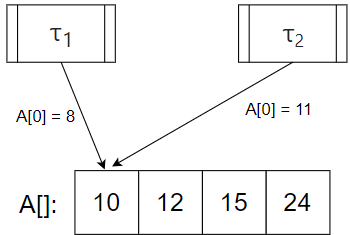
\includegraphics[width=0.4\textwidth]{images/shared_memory.png}
    \caption{An example of two processes writing to a shared in-memory array}
    \label{fig:shared_memory}
\end{figure}
\par
Elixir instead uses a message-passing model for IPC. More specifically, Elixir uses an actor-based model, where each process (actor) has its state and a message box to receive messages from other actors. Actors are responsible for sending a finite number of messages to other actors, spawning new actors and changing their behaviour based on the handling of messages received in the mailbox. Figure \ref{fig:actor_model} shows an example of how actors behave. The mailbox is not necessarily first in, first out (FIFO) but often implementations tend to be.
\begin{figure}[H]
    \centering
    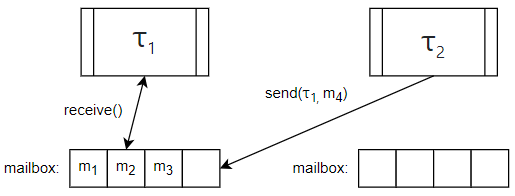
\includegraphics[width=0.6\textwidth]{images/actor_model.png}
    \caption{An example of actors sending and receiving messages under the actor model}
    \label{fig:actor_model}
\end{figure}
\par
In Elixir, a receive statement is used to read messages in the mailbox. The receive block looks through the mailbox for a message that matches a given pattern, if no messages match a given pattern, the process will block until one does.
\begin{lstlisting}[language=Elixir, xleftmargin=.4\linewidth, caption={An example of spawn/1 and spawn/4 in Elixir for spawning a new lightweight process and a new Elixir node}]
    # Example send in Elixir
    send self(), {:hello, "world"}

    # Example receive block in Elixir
    receive do
        {:hello, msg} -> IO.puts msg
    end
\end{lstlisting}
\section{Verifiable Feature Set} \label{sec:verifiable_feature_set}
In chapter \ref{chap:verlixir}, we will introduce Verlixir. Verlixir is designed to support a reduced set of core Elixir constructs. We will introduce these constructs here to give an overview of what the tool is capable of supporting.
\par
Everything in Elixir is an expression. This means that every piece of code returns a value. For example, an $if$ statement will return a value dependent on the branch taken. This means that any expression can be matched on, using Elixir's match (=) operator. We can use pattern matching to match on the shape of an expression's evaluation. The set of expressions supported by Verlixir are:
\begin{itemize}
    \item \textbf{Values}: any value of a basic, primitive type such as integers and booleans. Elixir also has a concept of $atoms$. An atom is identified by a preceding colon (:), and is followed by letters, digits, `\_', `@' or a string.
    \item \textbf{Variables}: Elixir is dynamically, strongly typed. Variables are bound to using the match operator. Variable names start with lowercase letters. The `\_' character can be used to match an expression of any shape.
    \item \textbf{Data structures}: structures such as lists and tuples are treated as values. Lists are dynamic, whereas tuples are fixed in size. Lists are written as [1, 2, 3] and tuples are written as \{1, 2, 3\}. We can match on the shape of these data structures using pattern matching.
    \item \textbf{Pattern matching}: pattern matching can be used to match on the shape of an expression. In the context of a conditional guard, values can be used to evaluate the shape of an expression, where as variables can be used to bind to the value of an expression. For example, the pattern ${:ok, value}$, can be used to assign to the variable $value$ if the expression is a tuple shape, with an atom $ok$ as the first element.
    \item \textbf{Functions}: functions are defined using the $def$ keyword. Functions can group multiple sequentially executable expressions. Any function can be called or spawned as a new process or node.
    \item \textbf{Modules}: functions are grouped into modules.
    \item \textbf{Message passing}: Elixir's actor model supports message passing. Messages are sent and received between actors and their mailboxes.
    \item \textbf{Control flow structures}: Elixir supports many control flow expressions. For example, $if$, $case$, $unless$ and $for$. All of these introduce a new scope. They are expressions and can be matched on.
\end{itemize}
\section{Summary}
In this chapter, we learned about Elixir, the programming language built on top of Erlang and we explored so basic approaches to designing concurrent systems with it. The next section will explore how these core tools can be used in tandem to provide developers guarantees over large-scale, distributed Elixir-based systems.